\documentclass[conference]{IEEEtran}
\IEEEoverridecommandlockouts
% The preceding line is only needed to identify funding in the first footnote. If that is unneeded, please comment it out.
\usepackage{cite}
\usepackage{amsmath,amssymb,amsfonts}
\usepackage{algorithmic}
\usepackage{graphicx}
\usepackage{textcomp}
\usepackage{xcolor}
\def\BibTeX{{\rm B\kern-.05em{\sc i\kern-.025em b}\kern-.08em
    T\kern-.1667em\lower.7ex\hbox{E}\kern-.125emX}}
\begin{document}

\title{Structural Machine Learning Homework}
\author{\IEEEauthorblockN{HO, WENHSIEN}}

\maketitle

\section{Data Preprocessing}
\subsection{Load The Data}
Build the dataset from the dataset file.
\begin{figure}[htbp]
\centerline{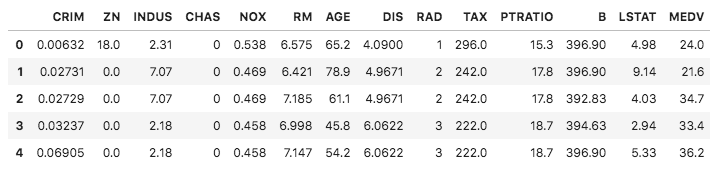
\includegraphics[width=9cm, height=4cm]{1.png}}
\caption{Housing dataset.}
\label{1}
\end{figure}
\subsection{Find Missing Data}
\begin{figure}[htbp]
\centerline{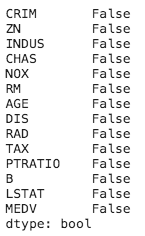
\includegraphics[width=3cm, height=5cm]{2.png}}
\caption{Find Missing Data.}
\label{2}
\end{figure}
\subsection{Apply Standarization to the features}
\begin{figure}[htbp]
\centerline{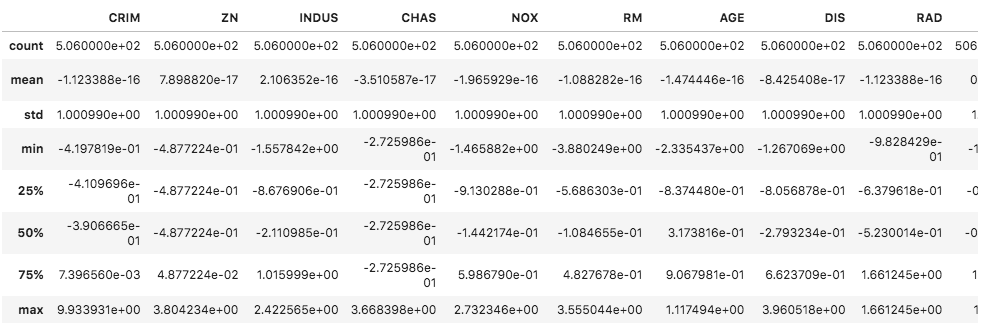
\includegraphics[width=9cm, height=4cm]{3.png}}
\caption{Standarization.}
\label{3}
\end{figure}
\subsection{Split the data}
\begin{figure}[htbp]
\centerline{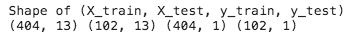
\includegraphics[width=8cm, height=1cm]{4.png}}
\caption{Shape of the training/testing data.}
\label{4}
\end{figure}




\section{Experimental Results}

\subsection{Cost}
\begin{figure}[htbp]
\centerline{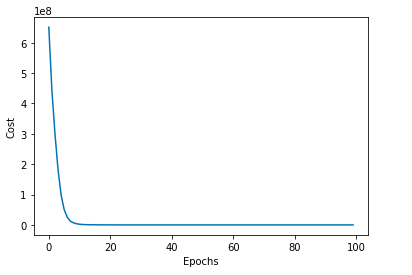
\includegraphics[width=7cm, height=5cm]{3-cost.png}}
\caption{Only 3-Layer MLP.}
\label{cost}
\end{figure}
\begin{figure}[htbp]
\centerline{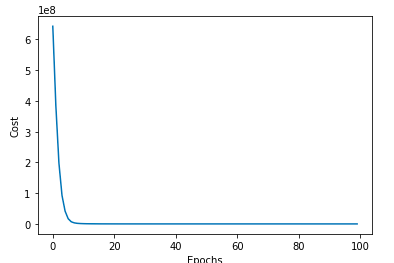
\includegraphics[width=7cm, height=5cm]{3-xav-cost.png}}
\caption{Apply Xavier Initialization.}
\label{cost_xav}
\end{figure}
\begin{figure}[htbp]
\centerline{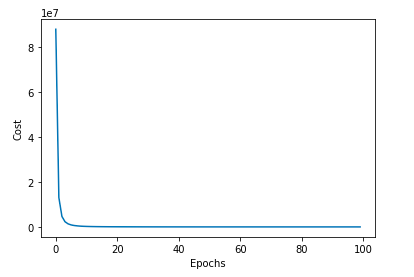
\includegraphics[width=7cm, height=5cm]{3-drop-cost.png}}
\caption{Apply Dropout.}
\label{cost_dropout}
\end{figure}
\newpage
\begin{figure}[htbp]
\centerline{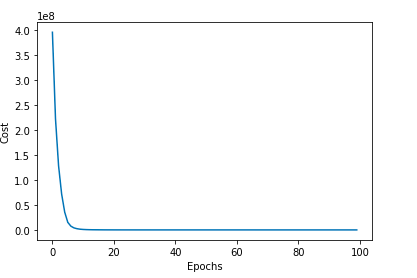
\includegraphics[width=7cm, height=5cm]{3-all-cost.png}}
\caption{Xavier Initialization + Dropout.}
\label{cost_all}
\end{figure}
\subsection{MSE}
\begin{figure}[htbp]
\centerline{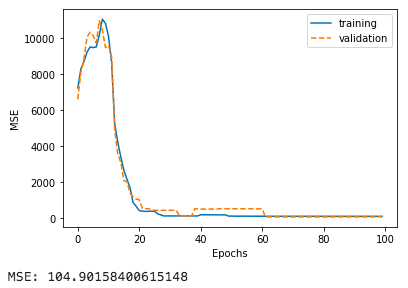
\includegraphics[width=7cm, height=5cm]{3-mse.png}}
\caption{Only 3-Layer MLP.}
\label{mse}
\end{figure}
\begin{figure}[htbp]
\centerline{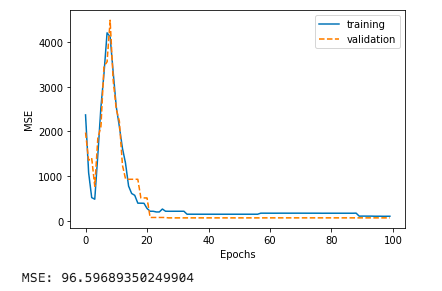
\includegraphics[width=7cm, height=5cm]{3-xav-mse.png}}
\caption{Apply Xavier Initialization.}
\label{mse_xav}
\end{figure}
\begin{figure}[htbp]
\centerline{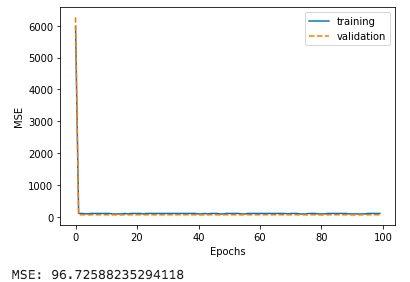
\includegraphics[width=7cm, height=5cm]{3-drop-mse.png}}
\caption{Apply Dropout.}
\label{mse_dropout}
\end{figure}
\newpage
\begin{figure}[htbp]
\centerline{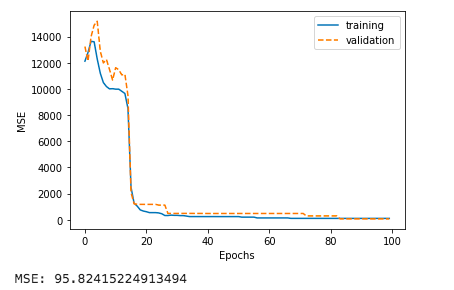
\includegraphics[width=7cm, height=5cm]{3-all-mse.png}}
\caption{Xavier Initialization + Dropout.}
\label{mse_all}
\end{figure}

\section{Conclusion}
In Figure 5-8, we found that there is no obvious difference in the cost part after applying Xavier Initialization and Dropout, but in Figure 9-12,we can see that mean square error significantly decreased when applying both Xavier Initialization and Dropout.

\end{document}

